\documentclass[tikz, preview]{standalone}

\usepackage{amsfonts, amsthm, amssymb, amsmath, stmaryrd, etoolbox}
\usepackage{tikz}
\usetikzlibrary{matrix,arrows}

\begin{document}
\[
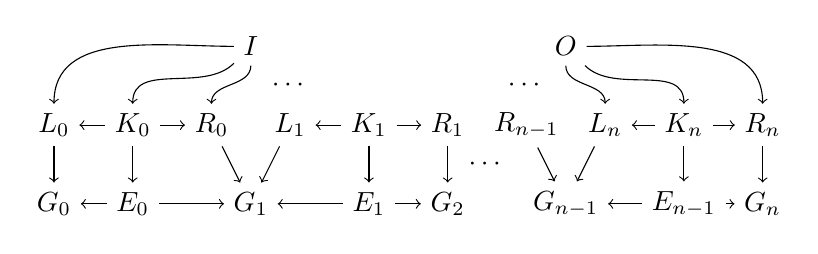
\begin{tikzpicture}
\node (G0) at (0,-1) {$G_0$};
\node (E0) at (1,-1) {$E_0$};
\node (G1) at (2.5,-1) {$G_1$};
\node (E1) at (4,-1) {$E_1$};
\node (G2) at (5,-1) {$G_2$};
\node (Gn-1) at (6.5,-1) {$G_{n-1}$};
\node (En-1) at (8,-1) {$E_{n-1}$};
\node (Gn) at (9,-1) {$G_n$};
\node (L0) at (0,0) {$L_0$};
\node (K0) at (1,0) {$K_0$};
\node (R0) at (2,0) {$R_0$};
\node (L1) at (3,0) {$L_1$};
\node (K1) at (4,0) {$K_1$};
\node (R1) at (5,0) {$R_1$};
\node (Rn-1) at (6,0) {$R_{n-1}$};
\node (Ln) at (7,0) {$L_n$};
\node (Kn) at (8,0) {$K_n$};
\node (Rn) at (9,0) {$R_n$};
\node (I) at (2.5,1) {$I$};
\node (O) at (6.5,1) {$O$};
\node (dots) at (5.5,-0.5) {$\dotsm$};
%
\draw [->] (L0) edge (G0);
\draw [->] (K0) edge (E0);
\draw [->] (R0) edge (G1);
\draw [->] (L1) edge (G1);
\draw [->] (K1) edge (E1);
\draw [->] (R1) edge (G2);
\draw [->] (Rn-1) edge (Gn-1);
\draw [->] (Ln) edge (Gn-1);
\draw [->] (Kn) edge (En-1);
\draw [->] (Rn) edge (Gn);
\draw [->] (K0) edge (L0);
\draw [->] (K0) edge (R0);
\draw [->] (K1) edge (L1);
\draw [->] (K1) edge (R1);
\draw [->] (Kn) edge (Ln);
\draw [->] (Kn) edge (Rn);
\draw [->] (E0) edge (G0);
\draw [->] (E0) edge (G1);
\draw [->] (E1) edge (G1);
\draw [->] (E1) edge (G2);
\draw [->] (En-1) edge (Gn-1);
\draw [->] (En-1) edge (Gn);
%
\draw [->] (I) edge[out=180,in=90] (L0);
\draw [->] (I) edge[out=225,in=90] (K0);
\draw [->] (I) edge[out=270,in=90] (R0);
\draw [->] (O) edge [out=0,in=90] (Rn);
\draw [->] (O) edge [out=-45,in=90] (Kn);
\draw [->] (O) edge [out=-90,in=90] (Ln);
%
\node (Idots) at (3,0.5) {$\dotsm$};
\node (Odots) at (6,0.5) {$\dotsm$};
\end{tikzpicture}
\]
\end{document}
